\section{Software Implementation}
SciKit-SurgeryFRED implements a simple user interface, Figure \ref{fig:surgery_fred}, to demonstrate registration of a pre-operative image to intra-operative space. At startup a target is placed at a random location within the pre-operative image, shown as a red circle. The standard deviation of the \gls{FLE} is randomly sampled from a uniform distribution 

\begin{figure}
	\begin{center}
	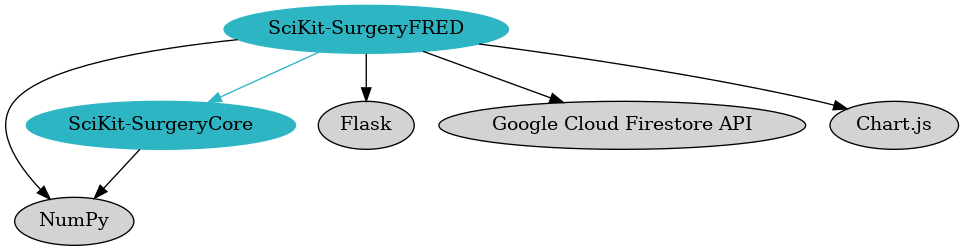
\includegraphics[width=0.7\linewidth]{dependency_graph.eps}
		\caption{\label{fig:dependencies}SciKit-SurgeryFRED graphical user interface after 3 fiducial markers placed. The red sphere in the pre-operative image (left) represents a clinical target, which is located in the
		intra-operative space (middle) by fiducial based registration, using the fiducial markers (green). FLE is added to each marker in the intra-operative image, this is more clearly visible on the zoomed in images at the right. The resulting registration results in a TRE, shown by the misalignment of the red circle and crosshair 
		on the enlarged image at right. TRE and other statistics are shown across the top
		of the window.}
	\end{center}
\end{figure}
\begin{pythonlisting}{Python to generate independent FLE}
if ind_fle_function is None:
    if independent_fle is None:
        independent_fle = 0.0
        ind_fle = _set_fle(independent_fle, dimension)
        def ind_fle_function():
        return np.random.normal(loc=0.0, scale=ind_fle, size=dimension)
    else:
        if independent_fle is not None:
            raise ValueError("Set independent_fle and ind_fle_function, ",
                             "independent_fle will be ignored")
    self.ind_fle_function = ind_fle_function
\end{pythonlisting}
	
\begin{javalisting}{Java to generate independent FLE}
function clearCanvas(canvas) {
  if (canvas.getContext) {
    var ctx = canvas.getContext('2d');
    ctx.clearRect(0, 0, canvas.width, canvas.height);
  }
}
\end{javalisting}

